
The handwriting recognition system has two levels of classifiers. 
The first classifier is a function that takes an image as input and outputs a character. 
The second classifier is a function that takes a string of characters as input and outputs a word. 
A flowchart that shows the classification process can be seen in figure~\ref{fig:classification_system_overview}. 

    \begin{figure}[htb] 
      \begin{center}
	\leavevmode
	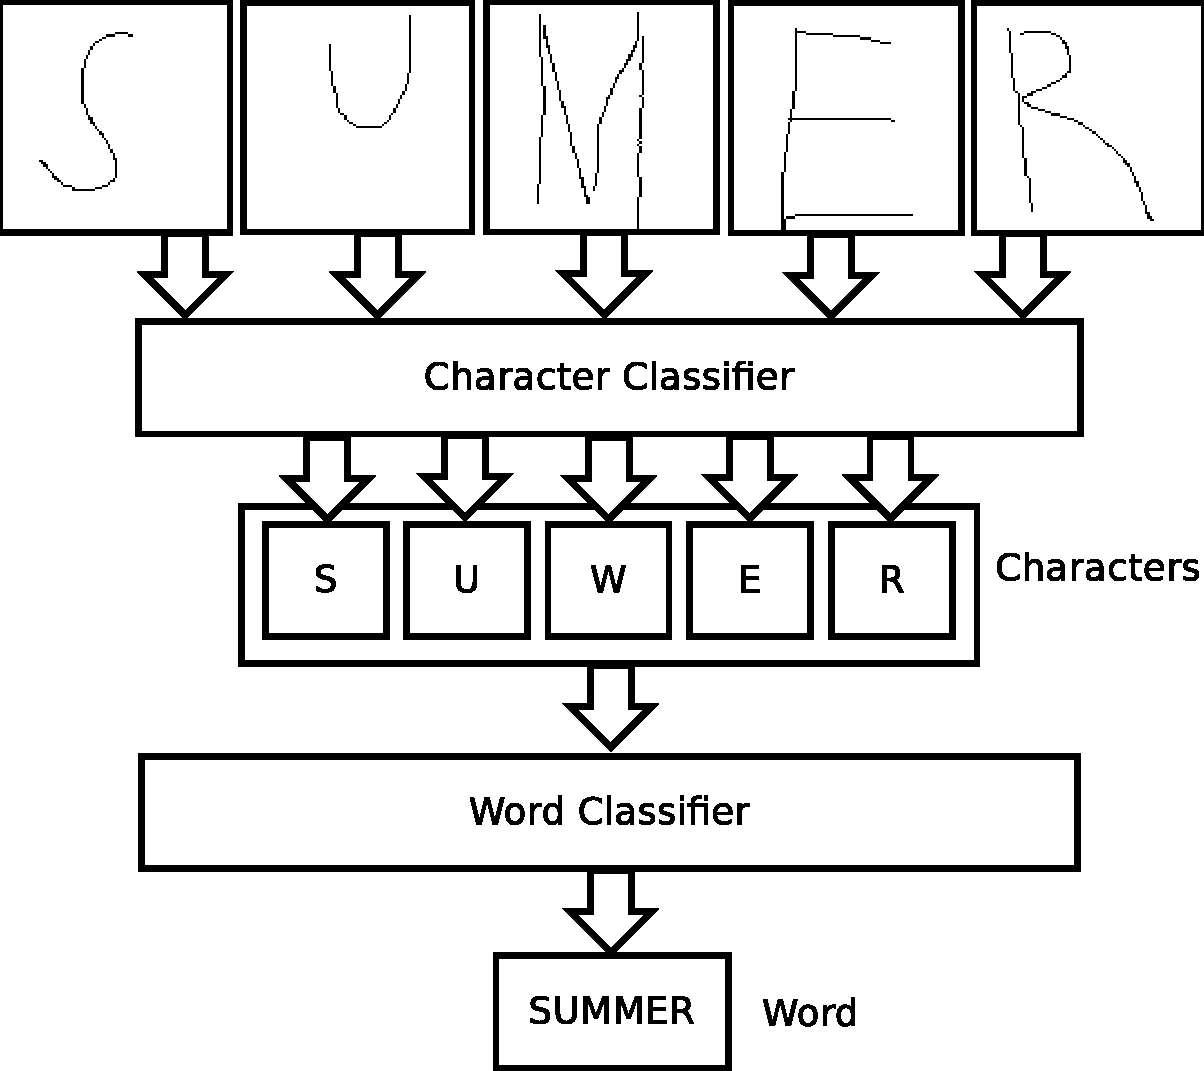
\includegraphics[width=110mm]{classification_system_overview.pdf}%width=115mm,height=40mm
      \end{center}
      \caption{Flowchart of classification process.}
      \label{fig:classification_system_overview}
    \end{figure}

The classifiers contains HMMs for all elements in the set of possible outputs. 
So if the character classifier is trained to recognize the 26 Latin characters, it will contain 26 HMMs. 
One HMM for every character. 
When the classifiers are trained they are given input examples for all possible outputs. 
If the input $I$ is given to one of the classifiers the following steps are performed to calculate the output:

\begin{enumerate}
  \item The probability of $I$ is calculated for all HMMs contained in the classifier:
    \begin{enumerate}
      \item $I$ is translated to a sequence of observation symbols $\mathbf{O} = O_{1},O_{2},...,O_{n}$. 
      If $I$ is a string of characters and the output of the classifier is a word, the translation is straightforward. 
      Every character in the string is simply translated to the corresponding observation symbol. 
      There are also special observations for the start and end states. 
      This is explained in more detail in the following sections. 
      If $I$ is an image, the image is first segmented to a sequence of segments. 
      An observation symbol is then obtained from all segments. 
      See section~\ref{sec:image_preprocessing} for more information about the image feature extraction.
      \item The forward calculation algorithm \cite{Rabiner1989} is then used to calculate the probability of $\mathbf{O}$ given the HMM.
    \end{enumerate}
  \item The output symbol with the highest probability in the previous step is returned as output.
\end{enumerate}
 
 %% I think this sentence should be split up or turned into a list. It's hard to read in its current form imo. --Fabian
The following parameters must be supplied when a classifier is created\footnote{A few more parameters can be given but are not listed here because of lack of importance. See the source code of the system for information about other parameters. How the source code can be obtained is explained in appendix~\ref{app:source_code}.}:
\begin{itemize}
 \item The set of possible output symbols and corresponding training examples.
 \item The initialization method that shall be used by the HMMs.
 \item If the training examples shall be used to train the model with the Baum-Welch \cite{Rabiner1989} training algorithm.
\end{itemize}
